\begin{frame}{Etablering af træ- og buskbevoksninger}

\small

\begin{columns}[T]

\begin{column}{0.58\textwidth}

\textbf{Regler for etablering af træ- og buskbevoksninger:}

\begin{itemize}[]
\item Max. 0,5 ha pr. tiltag
\item Min. 50 m mellem tiltag
\end{itemize}

\vspace{0.4em}

\textbf{Gavner arter:}

\footnotesize
Fasan, agerhøne, markhare, rådyr, dådyr, rødrygget tornskade, gul vipstjert, 
pirol, gulspurv, blåmejse, musvit, sortmejse, grønsisken, stillits, 
rødhals, flagermus, pindsvin, lækat, egern, musvåge, spurvehøg, tårnfalk

\end{column}

\begin{column}{0.40\textwidth}
\centering
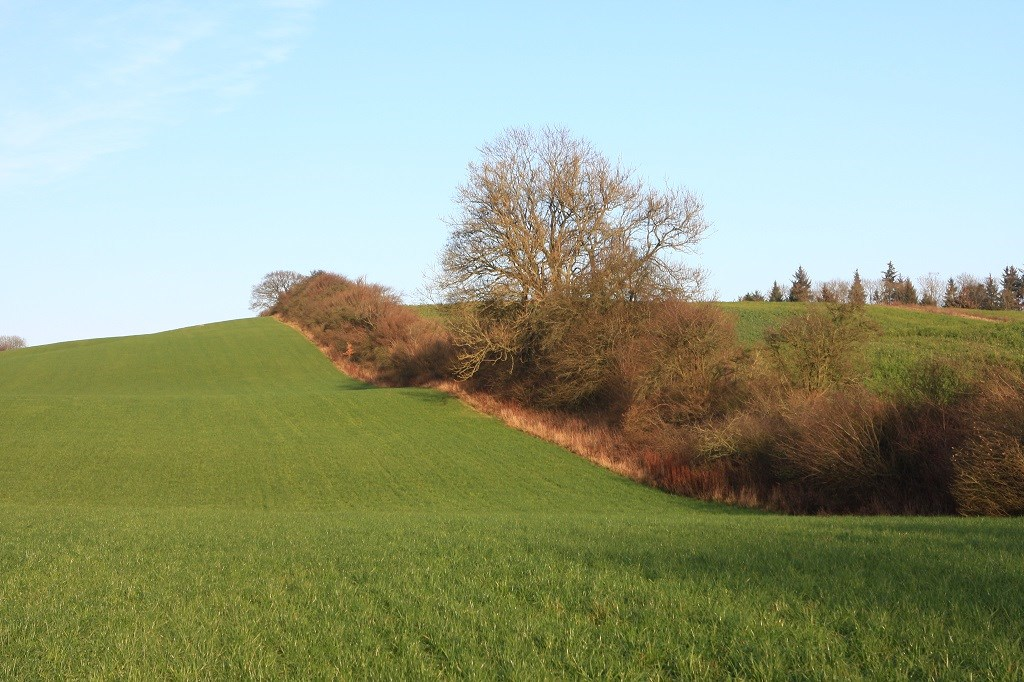
\includegraphics[width=\textwidth]{Billeder/Vildtforvaltning/biotopplantiltag/buskbevoksning.jpg}
\end{column}

\end{columns}

\end{frame}